%%%%%%%%%%%%%%%%%%%%%%%%%%%%%%%%%%%%%%%%%%%%%%%%%%%%%%%%%%%%%%%%%%%%%%%%%%%%%%%%%
%             __________________________________________________________        %
%            | FORMATION LATEX 2011 - A cube/ACELI/Louvain-li-Nux  |            %
%            |______________________- DAY 1 -__________________________|        %
%                                                                               %
%  • Document exemple avec des éléments de structure à reproduire               %
%  • Ce document est écrit avec des caractères encodés en utf8 :                %
%  les utilisateurs Windows qui souhaitent modifier ce document devront         %
%  soit     - changer l'encodage en [latin1] afin de pouvoir utiliser des       %
%                caractères spéciaux ou accents de leur clavier (il faudra dès  %
%                lors remplacer les accents/caractères spéciaux originaux du    %
%                document);                                                     %
%             - changer l'encodage par défaut des caractères dans l'éditeur     %
%                de texte utilisé en UTF-8.                                     %
%                                                                               %
%%%%%%%%%%%%%%%%%%%%%%%%%%%%%%%%%%%%%%%%%%%%%%%%%%%%%%%%%%%%%%%%%%%%%%%%%%%%%%%%%

\documentclass[12pt]{article} %% un article un 12
\usepackage[utf8]{inputenc}  % en règle générale - Windows : [latin1] - Linux/MacOS : [utf8]
\usepackage[T1]{fontenc}   %% encodage
\usepackage[french]{babel} %% langue
\usepackage{booktabs} %% tableau
\usepackage{graphicx} %% images
\usepackage{hyperref} %% liens
\usepackage{amsmath}
\usepackage{amssymb}
\usepackage{siunitx}

% \renewcommand{\familydefault}{\sfdefault} %% utilise la police SC, p-ê plus agréable

% \usepackage{float}              % nécessaire pour pouvoir utiliser l'option [H]  (figure ou table)

\author{Bill Murdock}
\title{Mon premier document \LaTeX}


\begin{document}
\maketitle

\tableofcontents
\newpage

\section{Introduction}
L'écriture de texte se fait très simplement. Chaque paragraphe est séparé par une ligne blanche dans le \verb|.tex| et l'indentation est automatique. De même, la césure \footnote{La rupture d'un mot en fin de ligne} et les numérotations sont gérées automatiquement qu'il s'agisse des numéros de pages, de tableaux, de figures ou encore des notes en bas de page.

\section{Problématique}

L'écriture mathématique peut s'écrire de plusieurs façons, nous en verrons ici deux, à savoir:
\begin{enumerate}
 	\item dans une ligne de texte.
      Par exemple, $A$ est une variable définie par $A=\sin(2x)$
 	\item sur une ligne séparée (voir section~\ref{eq}).
 \end{enumerate}

\subsection{Équations}\label{eq}

Les équations peuvent être référencées dans le texte facilement sans se préoccuper de la numérotation, un label pouvant être associé à chaque équation hors-ligne.
L'équation~\eqref{eq:pnorm} permet de déterminer la densité de probabilité d'une variable aléatoire suivant une loi normale.

\begin{align}
  \notag
  \sum_{i=1}^n i & =
  \begin{cases}
    \frac{n (n+1)}{2} & \text{si } i \geq 0\\
    0 & \text{sinon}
  \end{cases} & \forall i \in \mathbb{Z}\\
  \label{eq:pnorm}
  \mathsf{density}(x) & = \frac{1}{\sigma \sqrt{2\pi}} \exp \left(-\frac{(x-\mu)^2}{2\sigma^2}\right)
\end{align}

\subsection{Figures}

Les figures, comme décrit dans plusieurs sources dont \cite{codecco2001endemic}, se traitent comme des éléments flottants, vous pouvez préciser entre autre :
\begin{itemize}
	\item un titre,
	\item un label pour le référencement,
	\item un agencement particulier,
	\item une taille précise en cm ou \% de largeur de page de texte,
	\item une préférence sur le positionnement dans le document.
\end{itemize}

Néanmoins, \LaTeX{} reste seul juge sur l'emplacement de votre élément flottant (environnements \textbf{table} et \textbf{figure} par exemple).

% Attention, le nom du fichier image "image.png" est à remplacer par le nom d'une de vos images.
% L'image doit être présente dans le même dossier que ce fichier .tex
\begin{figure}[ht] % ou [!ht] pour forcer ([!]) à mettre l'image ici ([h]ere) ou alors en haut ([t]op)
	\centering
	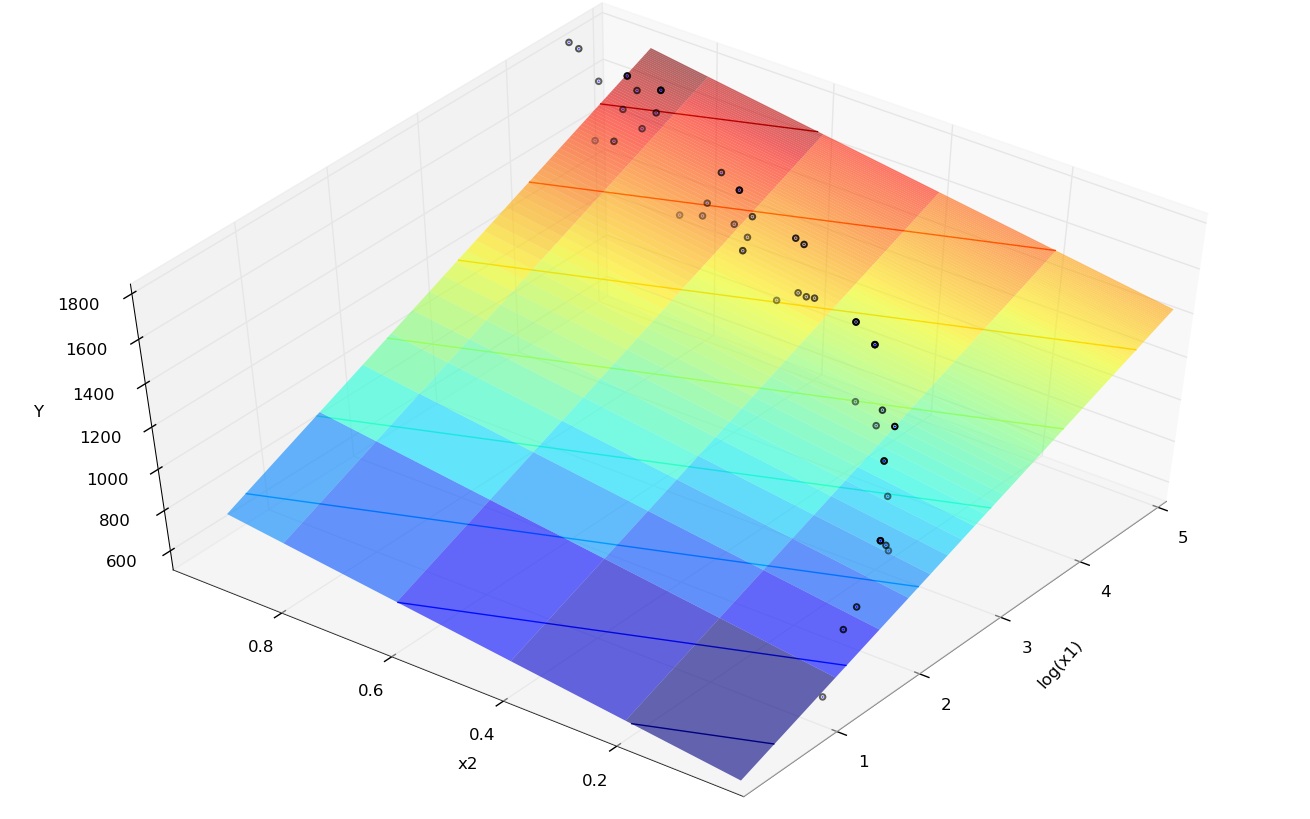
\includegraphics[width=\textwidth]{image.png}
	\caption{Régression linéaire multiple sur deux facteurs : $x_2$ et $\log(x_1)$.}
	\label{fig:image}
\end{figure}

\subsection{Analyse des données}

Le tableau~\ref{tab:env} est un exemple de tableau avec l'environnement \textbf{\textit{booktabs}}.

\begin{table}[!ht]
	\centering
	\begin{tabular}{lcc}
		\toprule
        \textbf{Sample Site} & \textbf{Temperature (\si{\celsius})} & \textbf{Gradient (\si{\degree})}\\
		\midrule
		Shakespeare & 22 & 5\\
		Wenderholm & 25 & 12\\
		Coromandel & 18 & 9\\
		\midrule
		\textbf{Average} & \textbf{21.7} & \textbf{8.7}\\
		\bottomrule
	\end{tabular}
    \caption{Environmental variables for several sample sites. The average is \SI{217e-1}{\celsius}.}
	\label{tab:env}
\end{table}

\bibliographystyle{plain}
\bibliography{biblio}

\end{document}
